% !TEX encoding = UTF-8 Unicode
\documentclass[a4paper]{article}

\usepackage{color}
\usepackage{url}
\usepackage[T2A]{fontenc} % enable Cyrillic fonts
\usepackage[utf8]{inputenc} % make weird characters work
\usepackage{graphicx}
\usepackage{amsmath}
\usepackage{mathtools}

\usepackage[english,serbian]{babel}
%\usepackage[english,serbianc]{babel} %ukljuciti babel sa ovim opcijama, umesto gornjim, ukoliko se koristi cirilica

\usepackage{epigraph}

\usepackage[unicode]{hyperref}
\hypersetup{colorlinks,citecolor=green,filecolor=green,linkcolor=blue,urlcolor=blue}

\usepackage{listings}

\graphicspath{ {./images/} }

%\newtheorem{primer}{Пример}[section] %ćirilični primer
\newtheorem{primer}{Primer}[section]

\definecolor{mygreen}{rgb}{0,0.6,0}
\definecolor{mygray}{rgb}{0.5,0.5,0.5}
\definecolor{mymauve}{rgb}{0.58,0,0.82}

\lstset{ 
  backgroundcolor=\color{white},   % choose the background color; you must add \usepackage{color} or \usepackage{xcolor}; should come as last argument
  basicstyle=\scriptsize\ttfamily,        % the size of the fonts that are used for the code
  breakatwhitespace=false,         % sets if automatic breaks should only happen at whitespace
  breaklines=true,                 % sets automatic line breaking
  captionpos=b,                    % sets the caption-position to bottom
  commentstyle=\color{mygreen},    % comment style
  deletekeywords={...},            % if you want to delete keywords from the given language
  escapeinside={\%*}{*)},          % if you want to add LaTeX within your code
  extendedchars=true,              % lets you use non-ASCII characters; for 8-bits encodings only, does not work with UTF-8
  firstnumber=1000,                % start line enumeration with line 1000
  frame=single,	                   % adds a frame around the code
  keepspaces=true,                 % keeps spaces in text, useful for keeping indentation of code (possibly needs columns=flexible)
  keywordstyle=\color{blue},       % keyword style
  language=Python,                 % the language of the code
  morekeywords={*,...},            % if you want to add more keywords to the set
  numbers=left,                    % where to put the line-numbers; possible values are (none, left, right)
  numbersep=5pt,                   % how far the line-numbers are from the code
  numberstyle=\tiny\color{mygray}, % the style that is used for the line-numbers
  rulecolor=\color{black},         % if not set, the frame-color may be changed on line-breaks within not-black text (e.g. comments (green here))
  showspaces=false,                % show spaces everywhere adding particular underscores; it overrides 'showstringspaces'
  showstringspaces=false,          % underline spaces within strings only
  showtabs=false,                  % show tabs within strings adding particular underscores
  stepnumber=2,                    % the step between two line-numbers. If it's 1, each line will be numbered
  stringstyle=\color{mymauve},     % string literal style
  tabsize=2,	                   % sets default tabsize to 2 spaces
  title=\lstname                   % show the filename of files included with \lstinputlisting; also try caption instead of title
}

\begin{document}

\title{Implementirano $\neq$ testirano $\neq$ ispravno\\ \small{Seminarski rad u okviru kursa\\Metodologija stručnog i naučnog rada\\ Matematički fakultet}}

\author{\normalsize{Nenad Ajvaz, Stefan Kapunac, Filip Jovanović, Aleksandra Radosavljević}\\
\normalsize{nenadajvaz@hotmail.com, stefankapunac@gmail.com,}\\
\normalsize{jovanovic16942@gmail.com, aleksandraradosavljevic.@live.com}
}

%\date{9.~april 2015.}

\maketitle

\abstract{
Softver igra sve veću ulogu u modernom svetu i stoga je sve važnije da on bude ispravan. Navešćemo primere katastrofalnih softverskih grešaka, a zatim ćemo prikazati različite metode za izbegavanje i uklanjanje takvih grešaka u različitim fazama razvoja. Posvetićemo pažnju i mogućnostima unapređenja procesa razvoja softvera koje nam donose nove tehnologije.
}

\tableofcontents

\newpage

\section{Uvod}
\label{sec:uvod}

U vreme ,,softverske krize‘‘ započet je razvoj na polju softverskog inženjerstva.
Programeri su radili na tome da isporuče što moćniji sistem i što efikasnije aplikacije, ali su nailazili na različite probleme, kao što su kašnjenje isporuka, troškovi veći od predviđenog, bagovi koje je teško ispraviti i još mnogo toga.
Softver danas ima značajnu ulogu u društvu i sve je rasprostranjeniji, te je njegova pouzdanost veoma relevantna, posebno ako se u obzir uzme prisutnost u zdravstvu, gde ima direktan uticaj na ljudske živote.

Razvoj softvera je disciplina koja se bavi proizvodnjom softvera, razvojnih alata, metodologija i teorema koje podržavaju razvoj.
Softverski inženjeri pri izradi prate proces od nekoliko koraka koji su prikazani na slici \ref{fig:rs}.
U nastavku ćemo se fokusirati na deo sa testiranjem, kao i njegovu vezu sa pouzdanošću softvera.
Pouzdanost softvera se definiše kao verovatnoća ispravnog rada sistema tokom određenog vremena, pri određenim uslovima \cite{pham_reliability}.
Malo neformalnije, pouzdanost je mera slaganja sistema sa svojom specifikacijom.

Da bismo istakli važnost pouzdanosti, počećemo, u poglavlju \ref{sec:primeri}, sa nekim primerima velikih problema koji su nastali zbog nepouzdanog softvera \cite{quinn_ethics}.
Potom ćemo se, u poglavlju \ref{sec:ispravnost}, baviti ispravnošću programa, kao osnovom pouzdanosti, gde ćemo zagrebati površinu oblasti verifikacije softvera \cite{laski2009software}.
Nakon toga ćemo, u poglavlju \ref{sec:modeli_metrike}, prikazati neke od modela i metrika koji se koriste u procenjivanju pouzdanosti softvera \cite{pham_reliability}.
Na kraju ćemo, u poglavlju \ref{sec:buducnost}, razmotriti moguća unapređenja celokupnog procesa razvoja softvera korišćenjem novih dostignuća na polju veštačke inteligencije.\\\\


\section{Primeri neispravnog softvera}
\label{sec:primeri}

Tokom proteklih decenija, tehnologija je doživela veliki napredak, ali usled grešaka u softveru je prouzrokovala velike materijalne gubitke, kao i ljudske žrtve. Kada započne sa radom i pokaže se ispravnim i odgovarajućim, očekuje se da će softver zadržati to svojstvo. Međutim, serije tragedija i haosa koje su uzrokovane padom softvera pokazuju suprotno.\\

\begin{primer}
\textbf{Therac-25, 1985.}
\end{primer}
Therac-25 je bila računarski kontrolisana mašina za terapiju zračenjem, proizvedena 1982.
Zbog grešaka u konkurentnom programiranju\footnote{ Višenitno programiranje, gde se skup sekvencijalnih programa izvršava paralelno.}, softver nije bio u stanju da detektuje određena stanja, a deo hardvera za interno zaključavanje, koji su prethodni modeli ove mašine posedovali i koji je služio da spreči ovakve greške ukoliko do njih dođe, otklonjen je i sve provere bezbednosti prepuštene su softveru. Ovaj propust je doveo do masovne pojave neodgovarajućih emisija zračenja.
Između juna 1985. i januara 1987. dogodilo se šest poznatih nesreća uzrokovanih predoziranjem zračenja koje su dovele do smrti i ozbiljnih povreda pacijenata. Prikaz mašine na slici \ref{fig:therac-25}.

\begin{figure}[h!]
\begin{center}
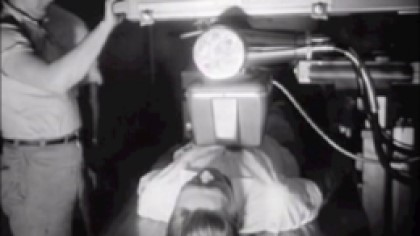
\includegraphics[scale=0.45]{therac}
\end{center}
\caption{Therac-25}
\label{fig:therac-25}
\end{figure}

\newpage

\begin{primer}
\textbf{Marsov orbiter za proučavanje klime, 1999.}
\end{primer}
Marsov orbiter za proučavanje klime (slika \ref{fig:mco}) je bila robotska svemirska sonda koju je \emph{NASA} \emph{(eng. National Aeronautics and Space Administration)} lansirala 11. decembra 1998. sa ciljem da istraži klimu i promene na površini Marsa. Kontakt sa sondom izgubljen je 23. septembra usled softverske greške, naime u računaru u kontroli misije na Zemlji koji je jedinicu za vrednost potiska\footnote{ Sila koja gura telo u suprotnom smeru od kojeg ga neke druge sile vuku, primer sila koja deluje na telo potopljeno u tečnost u suprotnom smeru od gravitacione sile.} izražavao američkim jedinicama (funtama u sekundi), umesto standardnim jedinicama SI sistema (njutnima u sekundi) kako je bilo ugovoreno između agencije \emph{NASA} i kompanije Lokid Martin. Usled toga je sonda pri ulasku u Marsovu orbitu išla trajektorijom koja je bila preblizu njegove površine i usled zagrevanja, prolaskom kroz gornje slojeve atmosfere se raspala.\\
Cena ove greške iznosila je oko \$125.000.000.

\begin{figure}[h!]
\begin{center}
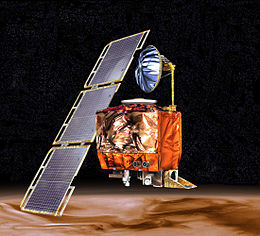
\includegraphics[scale=0.45]{MCO}
\end{center}
\caption{Marsov orbiter za proučavanje klime}
\label{fig:mco}
\end{figure}


\begin{primer}
\textbf{Letovi u Los Anđelesu}
\end{primer}
14. septembra 2004. godine, preko 400 aviona je izgubilo vezu sa kontrolom leta u blizini aerodroma u Los Anđelesu, međutim, zahvaljujući rezervnoj opremi unutar aviona, do nesreće nije došlo. Uzrok gubitka veze je bila greška prekoračenja u brojaču milisekundi u okviru sistema za komunikaciju sa avionima. Ova greška je bila otkrivena i pre incidenta, ali tada je sistem već bio isporučen i instaliran na nekoliko aerodroma, pa nije bilo moguće jednostavno ga popraviti i zameniti, već je preporučeno da se sistem resetuje na svakih 30 dana, kako ne bi došlo do prekoračenja. Ova procedura nije bila ispoštovana, i do greške je došlo posle tačno $2^{32}$ milisekundi, odnosno 49.7 dana od uključivanja sistema.\\

\begin{primer}
\textbf{Boing 737 MAX}
\end{primer}
Usled greške u softveru koji je ,,verovao‘‘ da je avion u opasnosti od iznenadnog gašenja motora i forsirao prednji deo aviona da počne da se spušta. Istražitelji su najveću pažnju posvetili proveri računarskog programa MCAS \emph{(eng. Maneuvering Charateristics Augmentation System)}, napravljen da pomogne pilotima da drže kontrolu nad avionima ovog tipa. Program reaguje kada senzori u kljunu aviona pokažu da se letelica penje pod prevelikim uglom, što može da dovede do gubitka kontrole. Piloti su se borili protiv sistema aviona ceo put i ispoštovali sve procedure pre pada aviona. Uprkos njihovim naporima, nisu uspeli da uspostave kontrolu nad letelicom i avion se srušio 10. marta 2019. i u nesreći je poginulo svih 157 osoba koje su bile u avionu, od kojih je jedna žrtva iz Srbije.\\


\section{Ispravnost programa}
\label{sec:ispravnost}
Greške u razvoju softvera su, kao i svuda, neizbežne. Ne može se očekivati visok nivo pouzdanosti softvera, ako se ne pokuša uklanjanje grešaka, koje se mogu javiti u bilo kom delu sistema. Dakle, kao što se vidi na slici \ref{fig:rs}, u razvojnom ciklusu softvera testiranje ima izuzetno važnu ulogu.

\begin{figure}[h!]
\begin{center}
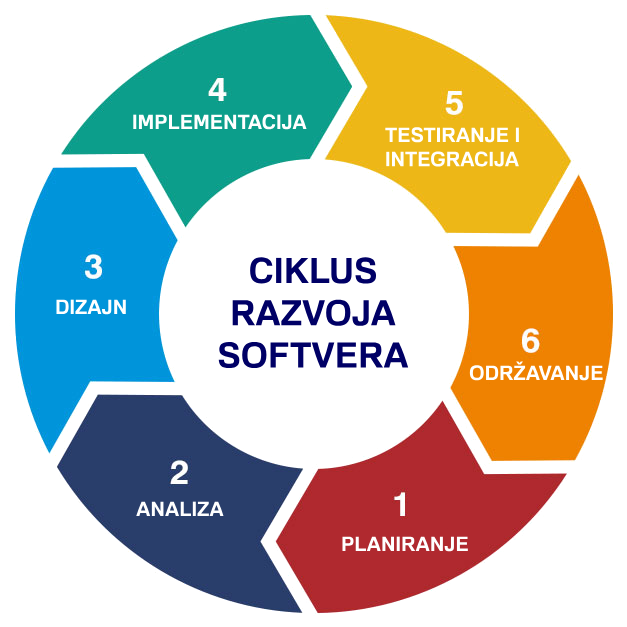
\includegraphics[scale=0.25]{rs.png}
\end{center}
\caption{Ciklus razvoja softvera}
\label{fig:rs}
\end{figure}

\subsection{Model problema i verifikacija softvera}
\label{subsec:ali}
\epigraph{\emph{,,Program testing can be used to show the presence of bugs, but never to show their absence!‘‘}}{Edsger W. Dijkstra}

Za skoro svaki, čak i najjednostavniji program postoji ogroman broj mogućih ulaznih vrednosti, tako da je iscrpno testiranje svih mogućnosti praktično neizvodljivo. Na primer, da bi se testiranjem dokazala ispravnost programa koji sabira dva 64-bitna broja, bi bi potrebno $2^{64} \cdot 2^{64}$ različitih testova. Uz pretpostavku da jedan test traje jednu nanosekundu, iscrpno testiranje bi trajalo $10^{22}$ godina. Testiranje je važno i podiže stepen pouzdanosti softvera, pomaže nam da uvidimo da postoje greške u programu, ali gotovo nikada se ne može samo testiranjem dokazati da one ne postoje.

Očigledno je potreban bolji pristup za dokazivanje ispravnosti programa. Grana računarstva koja se time bavi je verifikacija softvera.
Tačnije, proces verifikacije podrazumeva proveru da li program zadovoljava zadatu specifikaciju. Specifikacija predstavlja model problema i obično sadrži sledeće informacije \cite{laski2009software}:
\begin{itemize}
\item ulazni parametri
\item izlazni parametri
\item globalne promenljive kojima se može pristupiti
\item preduslovi - ograničenja na ulazne vrednosti
\item postuslovi - uslovi koje izlazne vrednosti moraju da zadovolje (za ulaze koji zadovoljavaju preduslove)
\end{itemize}
Verifikacija se sprovodi pod pretpostavkom da je specifikacija validna. Sa druge strane, validacija proverava da li specifikacija zadovoljava korisničke potrebe. Verifikacija i validacija se često, iako to nije tačno, izjednačavaju i poistovećuju sa testiranjem. Razliku između ova dva pojma na interesantan način objasnio je Beri Bem:
\begin{quote}
\emph{verification = Are we building the product right? \\
validation = Are we building the right product?}
\end{quote}

\subsection{Vrste verifikacije i njihov značaj za pouzdanost softvera}
\label{subsec:verifikacija}
Verifikacija softvera se u osnovi deli na dinamičku i statičku.\\
Dinamička verifikacija podrazumeva ispitivanje korektnosti programa u toku njegovog izvršavanja.
Najčešći oblik dinamičke verifikacije softvera jeste testiranje.\\
Najšira podela testiranja \cite{laski2009software}:
\begin{itemize}
\item testiranje crne kutije\\
Naziva se i funkcionalno testiranje.\\
Testovi se biraju na osnovu specifikacije.
\item testiranje bele kutije\\
Naziva se i strukturno testiranje.\\
Testovi se biraju na osnovu interne strukture koda.
\end{itemize}

Sa druge strane, statička verifikacija podrazumeva analizu izvornog koda programa, na osnovu koje se dolazi do zaključaka o njegovoj korektnosti.
Neke od metoda koje se koriste u statičkoj verifikaciji softvera su:
\begin{itemize}
\item simboličko izvršavanje \cite{symbolic_execution}\\
Koriste se simboličke promenljive umesto stvarnih ulaznih vrednosti, a kao izlaz se dobija simbolički izraz.
\item apstraktna interpretacija \cite{abstract_interpretation}\\
Posmatra se apstraktna semantika, nadskup konkretne semantike programa, u kojoj je rezonovanje jednostavnije.

\end{itemize}


\subsection{Formalni dokazi ispravnosti}
\label{subsec:formalni_dokazi}
Formalne metode verifikacije softvera podrazumevaju razvoj softvera direktno iz specifikacije i daju matematički dokaz korektnosti programa.
Uz programski k\^{o}d uporedo se formira i formalan matematički dokaz kojim se obezbeđuje ispravnost, bez potrebe za naknadnim testiranjem.
U te svrhe se koriste alati za interaktivno dokazivanje teorema, kao što su Isabelle/HOL \cite{isabelle} i Coq \cite{coq}.
Ovakvo rešenje je najbolje što se tiče pouzdanosti softvera, jer je matematički dokazana ispravnost.
Međutim, zbog potrebe za stručnjacima koji će to sprovoditi, povećavaju se troškovi, kao i trajanje razvojnog procesa, tako da ne čudi što se u industriji ove metode koriste samo u retkim slučajevima, i to samo za najkritičnije delove koda.\\
Neki od primera formalno verifikovanog softvera su:
\begin{itemize}
\item CompCert - kompilator za programski jezik C \cite{compcert}
\item seL4 - jezgro operativnog sistema (koristi se npr. u avio-industriji) \cite{sel4}
\item CakeML - implementacija programskog jezika ML sa formalno verifikovanim kompilatorom \cite{cakeml}
\item IronFleet - distribuirani sistemi \cite{ironfleet}
\end{itemize}

Radi ilustracije, u dodatku \ref{sec:dodatak} se nalazi primer dokaza algoritma quicksort iz dokumentacije Isabelle-a.


\subsection{Primer alata za testiranje - Selenium}
\label{subsec:primer_alata}
Selenium je skup softverskih alata koji služi da podrži i obezbedi sprovođenje automatskog i kontinuiranog testiranja softvera. Ovakav način testiranja obezbeđuje postojanu proveru funkcionalnosti i automatsko prijavljivanje nepravilnosti u radu softvera, što predstavlja veliku prednost u odnosu na manuelno testiranje softvera.\\

U osnovi Selenium je alat koji obezbedjuje automatizaciju internet pretraživača. To znači da pomoću njega možemo upravljati radom pretraživača, kontrolišući njihovo ponašanje i akcije koje će unutar pretraživača biti inicirane. Selenium skripte sadrže tipski grupisane akcije i iteracije nad pretraživačima i obezbeđuju njihovo automatizovano izvršavanje, što se u praksi koristi i za automatizaciju zadataka koji se često ponavljaju ili u svrhu kontinuiranog testiranja softvera. Prema podacima matičnog sajta \cite{Selenium}, Selenium predstavlja najzastupljenije rešenje otvorenog  k\^{o}da u oblasti automatizovanog testiranja.\\

Selenium je multiplatformsko rešenje u pravom smislu te reči. Podržan je rad sa svim trenutno bitnim veb pretraživačima, kao i pisanje testova u nekom od sledećih programskih jezika: Java, C\#, Ruby, Python, Perl i PHP. Ovaj fleksibilni alat može se koristi samostalno, kao i u kombinacija sa drugim test frejmvork platformama\footnote{ Frejmvork \emph(eng. framework) obezbeđuje već implementirane funkcionalnosti koje se mogu proizvoljno menjati od strane programera, uz značajnu uštedu vremena.}. Poseduje mogućnost brze i lake integracije sa mnogim eksternim alatama i API-jima. Inicijalna verzija Selenium-a pojavila se 2004 godine, a trenutno je aktuelna verzija 2.45.0. U pitanju je rešenje koje je u potpunosti otvorenog  k\^{o}da, razvijen je pod Apache licencom verzije 2.

\section{Modeli i metrike pouzdanosti softvera}	
\label{sec:modeli_metrike}

Prilikom izgradnje softvera, veoma je važno imati na umu da se greška može naći u bilo kojoj fazi njegovog razvoja. Zato je bitno da se pronađe način procene broja potencijalnih grešaka u sistemu.

Statistika pokazuje da se krajem 20. veka na 1000 linija koda pojavi oko 8 grešaka, ne računajući prethodno testiranje sistema. Različiti izvori napominju da je danas taj broj veći, nabraja se 15-50 grešaka na 1000 linija. Majkrosoft tvrdi da njihov k\^{o}d sadrži 0.5 neispravnosti na istom broju linija, dok \emph{NASA} čak ni na 500,000 linija programskog koda ne sadrži niti jedan softverski problem \cite{Statistika_prosek_gresaka}. Ovi brojevi su rezulat mnogih spoljašnjih faktora i nisu odgovarajuće merilo propusta i grešaka. Zbog toga su napravljeni razni modeli i metrike koji preciznije daju informaciju o stabilnosti softvera. U nastavku će biti opisana dva tipa takvih modela.\\


\subsection{Deterministički modeli}
\label{sec:deterministicki}

Ovi modeli odlikuju preciznim merama i podacima koji se oslanjanju na same karakteristike programskog koda. Prilikom ocenjivanja, ne uzimaju se u obzir slučajni događaji i greške koje oni prouzrokuju, već su performanse računate prema egzaktnim podacima. Oni uključuju broj različitih operatora, operanada, kao i broj mašinskih instrukcija i grešaka. Fokus je na mehanizmu i načinu rada samog softvera, gde se uvek mogu predvideti očekivana stanja.\\
Dva najpoznatija deterministička modela su Holstedova metrika i Mek-Kejbova ciklomatična složenost\footnote{ Moris Hauard Holsted (1977), Tomas Mek-Kejb (1976)}.

\subsubsection{Holstedova metrika}
\label{subsec:holsted}

Ova metrika se smatra jednom od najboljih za procenu kompleksnosti softvera, ali i težinu prilikom njegovog testiranja i debagovanja. U obzir ocene implementacije ulazi broj instrukcija i operacija izvornog koda, koji će biti drugačiji za svaki programski jezik ili arhitekturu na kojoj se program izvršava. Uvodi se sledeća notacija:
\begin{table}[h]
\centering
 \begin{tabular}{|c|c|c|}
  \hline
  Obeležje & Opis & Formula \\ [0ex]
  \hline $n_1$ & broj jedinstvenih operatora & \\ 
  \hline $n_2$ & broj jedinstvenih operanada & \\ 
  \hline $n$ & vokabular programa & $ n_1 + n_2 $ \\ 
  \hline $N_1$ & ukupan broj operatora & $ n_1 \cdot log_2(n_1) $ \\ 
  \hline $N_2$ & ukupan broj operanada & $ n_2 \cdot log_2(n_2) $ \\ 
  \hline $N$ & dužina programa & $ N_1 + N_2 $ \\
  \hline $I$ & broj mašinskih instrukcija & \\
  \hline $V$ & obim programa & $ N \cdot log_2(n_1+n_2) $ \\
  \hline $D$ & težina razumevanja i debagovanja & $ n_1/2 \cdot N_2 / 2  $ \\
  \hline $M$ & vreme utrošeno na implementaciju & $ V \cdot D $ \\
  \hline $T$ & vreme utrošeno na testiranje & $ M / 18 $ \\
  \hline $E$ & broj grešaka i bagova & $ V / 3000 $ \\
  \hline
 \end{tabular}
 \caption{Obeležja u Holstedovoj metrici. Brojevi su dobijeni empirijski \cite{ibm_halstead}}
 \label{tabela:1} 
\end{table}

\subsubsection{Mek-Kejbova ciklomatična složenost}
\label{subsec:mekkejb}

Ova metrika računa složenost dijagrama koji se pravi na osnovu grafa kontrole toka podataka programa. Čvorovi grafa predstavljaju različite komande, a oni su povezani usmerenom granom ako je sledeća naredba prvog čvora ona naredba u drugom čvoru. U slučaju da je graf povezan, ciklomatični broj jednak je broju linearno nezavisnih putanja kroz graf. Jednostavnije rečeno, ako program ne sadrži uslove i grananja, taj broj je 1. Zatim bi se taj broj povećao za 1 svaki put kada se naiđe na neku od ključnih reči: if, while, for, repeat, and, or itd. U naredbi case bi se svaki slučaj posebno računao.\\
Mek-Kejb je za Fortran okruženje odredio da je gornja granica za ciklomatični broj 10, i program se u tom slučaju može smatrati visokog kvaliteta.\cite{mccabe_fortran}\\\\
Ovom metrikom se mogu meriti i manje celine izvornog koda, kao što su pojedinačne funkcije, klase, moduli i potprogrami.\\
Ciklomatični broj C(G) grafa G se računa po formuli:
\begin{center}
C(G) = E - V + 2P,
\end{center}
gde je:\\
E = broj grana grafa\\
V = broj čvorova grafa\\
P = broj povezanih komponenti grafa\\

Ciklomatični broj grafa sa više od jedne povezane komponente se računa kao suma ciklomatičnih brojeva svakih od povezanih komponenti. Kada se merenje vrši nad funkcijom,  P će biti 1, jer funkcija predstavlja jedinstvenu povezanu komponentu.\\

\subsection{Probabilistički modeli}
\label{sec:probabilisticki}

Ovi modeli pojavu grešaka i kvarova gledaju kao na verovatnosne događaje. Softver se posmatra u fazi izvršavanja i pravi se mreža modela koja predstavlja ponašanje programa. Rezultat ovog modeliranja je primenjiv na razne metode iz oblasti statistike, što omogućava dubinsku matematičku analizu, detekciju anomalija, generisanju testova i simulaciju raznih slučajeva. Postoji nekoliko probabilističkih modela, od kojih će u nastavku biti opisana dva proizvoljna. \\

\subsubsection{Modeli stope neuspeha}
\label{subsec:stopa_neuspeha}

Ova grupa modela se koristi radi prikazivanja kolika je stopa otkazivanja programa po grešci. Kako se broj preostalih grešaka menja, tako se i stopa neuspeha prilagođava promeni.

Postoji nekoliko varijacija ovih modela, ali se svi oslanjaju na princip da u kodu postoji \textit{N} međusobno nezavisnih grešaka sa jednakom verovatnoćom ispoljavanja. Kada ona nastane, greška se otklanja i nijedna nova greška se ne pojavljuje prilikom uklanjanja.
Razlika je u tome što neki podmodeli podrazumevaju povećanje broja grešaka kroz vreme, drugi podrazumevaju smanjenje, a neki ga smatraju konstantnim. Takođe postoje modeli koji sa sigurnošću tvrde da je greška uklonjena, a postoje i oni koji uspešnost otklanjanja procenjuju verovatnoćom \textit{p}.

\subsubsection{Modeli rasta pouzdanosti}
\label{subsec:rast_pouzdanosti}

Ova grupa modela predviđa da li će doći do poboljšanja pouzdanosti kroz testiranje softvera. Model rasta je zapravo odnos pouzdanosti i stope neuspeha programa predstavljen kao funkcija vremena ili kao broj testova.\\
Postoje dva podmodela: prvi dovodi u korelaciju broj pronađenih i razrešenih grešaka, ukupni akumulirani broj grešaka u vremenskoj jedinici, dok drugi predviđa broj grešaka za vreme testiranja u jedinici vremena. U ovom modelu je najčešća vremenska jedinica jedna nedelja.


\section{Budućnost softvera}
\label{sec:buducnost}

Sa poboljšanjem hardvera, mogućnosti softvera postaju sve veće. Pomaci u oblastima veštačke inteligencije i mašinskog učenja omogućavaju mašinama da zamene ljude u nekim delatnostima, što donosi mnoge prednosti kao što su ubrzanje rada, smanjenje troškova i uklanjanje grešaka koje ljudi prave.

\subsection{Veštački programeri - fantastika ili realnost?}
Postoje mnogi programerski alati koji pomažu programerima tako što vrše automatsko generisanje koda, optimizaciju  ili debagovanje.
Sa napretkom veštačke inteligencije, mogućnost automatizacije raznih faza razvoja softvera raste.

Naravno, ideja da će računar sam da napiše komplikovan program je naučna fantastika. Da bismo napravili model koji će da napiše neki program, često nam je potrebno više posla nego da sami napišemo taj program. Međutim, programeri danas retko pišu ceo k\^{o}d od početka do kraja. Najčešće koristimo razne biblioteke i API-je, koji se konstantno menjaju, unapređuju, a i pišu novi. Učenje novih API-ja postaje iscrpljujuće za programera, te nastaje potreba za sistemima koji bi, za određeni ulaz programera, zaključili šta je zadatak i generisali gotov k\^{o}d. Jedan takav sistem je Bayou \cite{bayou}. Njegove mogućnosti su veoma ograničene, ali sa novim poboljšanjima na polju mašinskog učenja i veštačke inteligencije, možemo očekivati sve više takvih sistema u budućnosti.

Ova oblast tek počinje da se razvija, pa napredni sistemi tog tipa, ako postoje, nisu dostupni široj javnosti. Jasno je da ako je sistem ispravan, generisaće ispravne programe. Međutim, verifikacija sistema koji se trenira mašinskim učenjem nije jednostavna, a ni moguća u svim slučajevima. Programe dobijene na ovakav način će biti neophodno verifikovati i najverovatnije modifikovati, ali će proces razvoja biti znatno ubrzan upotrebom veštačke inteligencije. 

\section{Zaključak}
\label{sec:zakljucak}
Na osnovu svega navedenog, zaključujemo da u razvoju softvera nije dovoljno poznavati samo programski jezik i biti vešt u programiranju,
već je neophodno imati duboke uvide u domen primene.
Najbolje bi bilo da sve što implementiramo i formalno dokažemo.
Međutim, kako je to najčešće neizvodljivo, tj. neisplativo, moramo se ozbiljno posvetiti praćenju i održavanju nivoa pouzdanosti softvera
na neki drugi, ,,jednostavniji'' način, poput testiranja.
Moramo biti svesni da će do grešaka doći. 
Biće nam lakše da se na to pripremimo i adekvatno odreagujemo kada do greške dođe
ako unapred znamo koji delovi su podložni padovima i sa kojom verovatnoćom.
Očekujemo da će u budućnosti mnogi koraci razvoja biti automatizovani pre svega upotrebom veštačke inteligencije, ali i drugih metoda.

\addcontentsline{toc}{section}{Literatura}
\appendix
\bibliography{seminarski} 
\bibliographystyle{ieeetr}

\clearpage

\appendix
\section{Dodatak}
\label{sec:dodatak}
Algoritam sortiranja quicksort implementiran je na prirodan način za funkcionalni programski jezik.
Njegova korektnost dokazana je pomoću matematičke indukcije, koristeći ugrađene automatske dokazivače teorema uz pomoć nekih već dokazanih svojstava sortiranih lista.

\begin{lstlisting}[caption={Isabelle dokaz korektnosti algoritma quicksort}]
(*  Author:     Tobias Nipkow
    Copyright   1994 TU Muenchen
*)

section <Quicksort with function package>

theory Quicksort
imports "HOL-Library.Multiset"
begin

context linorder
begin

fun quicksort :: "'a list => 'a list" where
  "quicksort []     = []"
| "quicksort (x#xs) = quicksort [y<-xs. \<not> x\<le>y] @ [x] @ quicksort [y<-xs. x\<le>y]"

lemma [code]:
  "quicksort []     = []"
  "quicksort (x#xs) = quicksort [y<-xs. \<not> x\<le>y] @ [x] @ quicksort [y<-xs. x\<le>y]"
  by (simp_all add: not_le)

lemma quicksort_permutes [simp]:
  "mset (quicksort xs) = mset xs"
  by (induct xs rule: quicksort.induct) (simp_all add: ac_simps)

lemma set_quicksort [simp]: "set (quicksort xs) = set xs"
proof -
  have "set_mset (mset (quicksort xs)) = set_mset (mset xs)"
    by simp
  then show ?thesis by (simp only: set_mset_mset)
qed

lemma sorted_quicksort: "sorted (quicksort xs)"
  by (induct xs rule: quicksort.induct) (auto simp add: sorted_append not_le less_imp_le)

theorem sort_quicksort:
  "sort = quicksort"
  by (rule ext, rule properties_for_sort) (fact quicksort_permutes sorted_quicksort)+

end

end
\end{lstlisting}


\end{document}
